\chapter{Microbit Neural Network - python}

\section{without the microbit}
\subsection{Overview:}
The characteristics of the system will be:
Inputs are going to be binary
Weighted sum is bias+W1*input1+w2*input2
If weighted sum>=0 then the output is True (T on the LEDs) or '1'
If weighted sum<0 then the output is False (F on the LEDs) or '0

subsection{Single Neuron (without the Microbit)}
Lets start without the microbit and build a single neuron in Python and useful exercise in it's own right just to see the mechanism. A class Neuron is produced and all possible combination of a two-input binary system are feed in. 
\begin{verbatim}
class Neuron:
    def __init__(self, input1, bias, w1, w2):
        self.input1 = input1
        self.bias = bias
        self.w1=w1
        self.w2=w2
    
    def CalculateOutput (self):
        output1 = 0
        net = self.bias+self.input1[0]*self.w1+self.input1[1]*self.w2
        if net >= 0:
            output1 = 1
        else:
            output1 = 0
        return output1


for x1 in range (2):
    for x2 in range (2):
        neuron1= Neuron([x1,x2],-1,1,1)

        print("x1="+str(x1)+"x2= "+str(x2)+" Output= " +str(neuron1.CalculateOutput()))
\end{verbatim}


The code above implements a simple single neuron and the weights -1,1,1 produce an OR gate and -2,1,1 produces an AND gate.

\subsection{A Neural Network}
We can extend the code above to produce a neural network, by feeding the outputs of one or more neurons as inputs to other neurones. The code below produces an Exclusive XOR - essentially for the two input case if the two inputs are different then the output is True. The same inputs go to two neurones but they have different weight (bias, W1 and W2) but the outputs from these neurones are the inputs to a third neurone. The code is shown below (the Neuron class hasn't changed):
\begin{verbatim}
    class Neuron:
    def __init__(self, input1, bias, w1, w2):
        self.input1 = input1
        self.bias = bias
        self.w1=w1
        self.w2=w2
    
    def CalculateOutput (self):
        output1 = 0
        net = self.bias+self.input1[0]*self.w1+self.input1[1]*self.w2
        if net >= 0:
            output1 = 1
        else:
            output1 = 0
        return output1


for x1 in range (2):
    for x2 in range (2):
        neuron1= Neuron([x1,x2],-1,-1,1)
        neuron2= Neuron([x1,x2],-1,1,-1)
        neuron3= Neuron([neuron1.CalculateOutput(),neuron2.CalculateOutput()],-1,1,1)
        print("x1="+str(x1)+"x2= "+str(x2)+" Output 1= "+str(neuron1.CalculateOutput())+" Output 2= "+str(neuron2.CalculateOutput())+" Output overall= "+str(neuron3.CalculateOutput()))
\end{verbatim}


        



\section{with the microbit}
This is second in a two-post series on building a neural network using microbits with micropython. 
In the first post python was used to produce a neural network without the microbits. 

In this post the network is as shown in figure 1 is developed.

The figure below shows the arrangement of the connections to be built; pin 2 is the output of each neuron. 

The two micro:bits/neurons on the left of the picture taking in the two same inputs; the output from these neurons are the two inputs to the output neuron on the right.

The micro:bit objects used in Figure 1 were produced using the micro:bit Fritzing diagram available at 
\url{https://github.com/microbit-foundation/dev-docs/issues/36} thanks to David Whale (@whalleygeek ) for this.

\begin{figure}
    \centering
    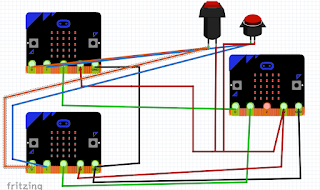
\includegraphics[width=10cm]{chapters/chAi1/figures/Screen Shot 2018-04-03 at 14.08.07.png}
    \caption{Microbit neural network}
    \label{fig:MicroibitANN1}
\end{figure}

\section{The Inputs neurons}

Neuron 1:

\begin{verbatim}
from microbit import *
W=[-1,-1,1]
while True:
    x1=pin0.read_digital()
    x2=pin1.read_digital()
    net = W[0]+W[1]*x1+W[2]*x2
    if net>=0:
        display.scroll("T")
        pin2.write_digital(1)
    else:
        display.scroll("F")
        pin2.write_digital(0)
\end{verbatim}


Neuron 2
\begin{verbatim}
from microbit import *
W=[-1,1,-1]
while True:
    x1=pin0.read_digital()
    x2=pin1.read_digital()
    net = W[0]+W[1]*x1+W[2]*x2
    if net>=0:
        display.scroll("T")
        pin2.write_digital(1)
    else:
        display.scroll("F")
        pin2.write_digital(0)   
\end{verbatim}




\section{Output Neuron.}
Feeding the inputs from Neuron 1 and Neuron 2 as inputs

\begin{verbatim}
from microbit import *
W=[-1,1,1]
while True:
    x1=pin0.read_digital()
    x2=pin1.read_digital()
    net = W[0]+W[1]*x1+W[2]*x2
    if net>=0:
        display.scroll("T")
        pin2.write_digital(1)
    else:
        display.scroll("F")
        pin2.write_digital(0)  
\end{verbatim}






